\subsection{Problema abordado}
\label{sec:problema}

\textcolor{red}{Descrição do problema a ser resolvido, uma condição a ser aprimorada ou produto desenvolvido.}

\textcolor{red}{Procure justificar seu problema com clareza, trazendo dados sobre a importância dele e sobre a necessidade das pessoas para que seja resolvido. Um problema bem definido  precisa ser:
\begin{itemize}
    \item Escrito em termos humanos (ao invés de tecnologia, produto ou funcionalidade de serviço);
    \item Abrangente o suficiente para permitir que você descubra áreas de valor inesperado;
    \item Específico o suficiente para ser gerenciável;
    \item Em formato de pergunta começando com “Como podemos..."
\end{itemize}}

\textcolor{red}{Procure ainda posicionar o problema em relação às diretrizes municipais, estaduais, nacionais e/ou mundiais. Exemplo: o problema está relacionado com uma das metas da ONU? o problema está previsto no plano diretor de uma secretaria de estado?}

\textcolor{red}{\textit{Por exemplo, desenvolvimento de um sistema de radar de carros que monitorem a velocidade dos carros em estacionamentos, pequenas vilas ou locais onde os carros tenham um limite de velocidade preestabelecido. (Este exemplo é bem sucinto e o grupo pode descrever mais aqui. Um problema claramente descrito significa menos dor de cabeça na execução do projeto! O escopo do  problema é definido principalmente nesta seção).}}

\textcolor{red}{
Nesta seção você deve ter referências dando suporte ao seus argumentos. Para citar, inclua o bibtex do material que deseja citar no arquivo "referencias.bib" e use o comando "cite" da forma que fazemos a seguir \cite{lee2020deep}. Neste sentido é importante lembrar que um projeto é um documento focado e que nele não há espaço para uma seção de bibliografia (geralmente comum em textos mais longos como livros), mas apenas podemos colocar referências bibliográficas, que coletam aqueles materiais que foram efetivamente usados ao longo do texto.}

\textcolor{red}{Notas de rodapé podem ser usadas para indicar comentários ou um site, por exemplo.\footnote{\url{http://www.ufpa.br}}}

\textcolor{red}{Nesta seção, você pode trazer figuras e tabelas para ilustrar o problema. A Figura \ref{fig:exemplo} e a Tabela \ref{tab:exemplo} mostram como fazer isso. Use estes \textit{templates} para adicionar outras figuras e tabelas.}

\begin{figure}[ht]
\centering
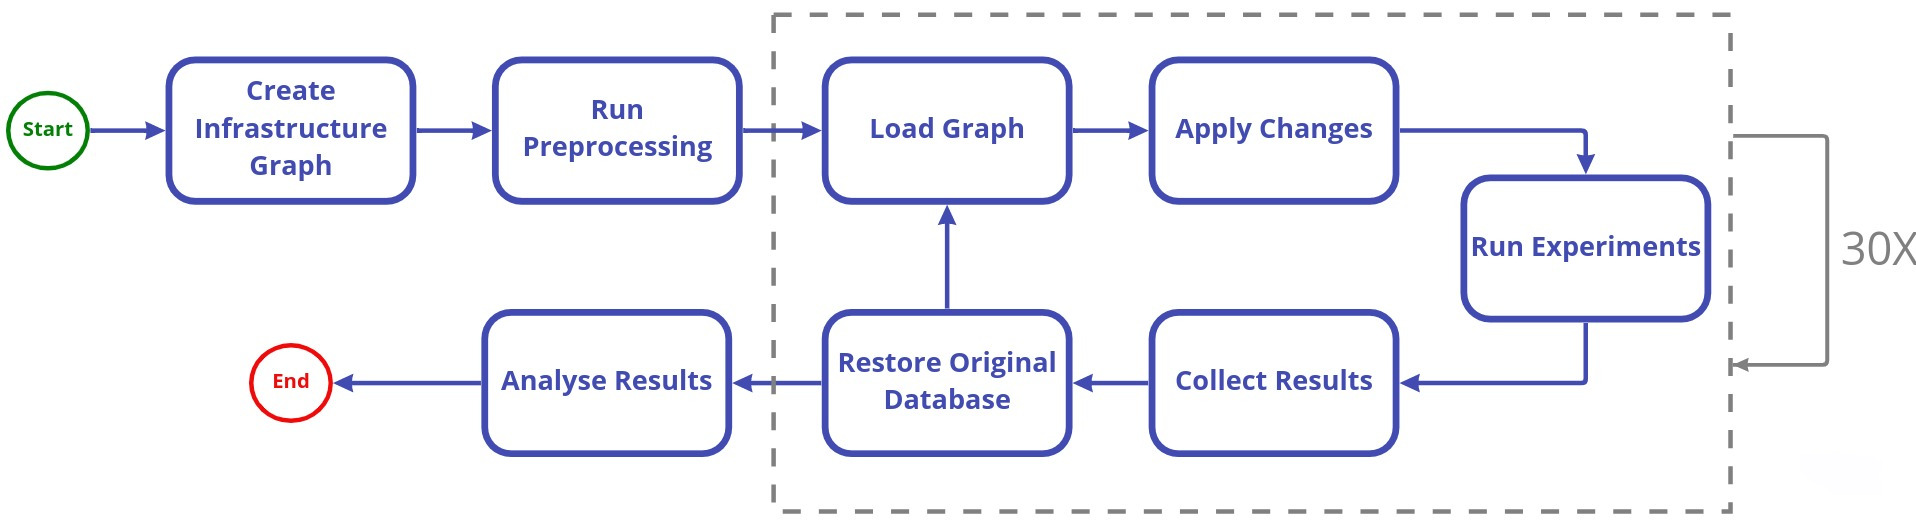
\includegraphics[width=0.9\textwidth]{figures/methodology.jpg}
\caption{Figura de exemplo}
\label{fig:exemplo}
\end{figure}


\begin{table}[ht]
\centering
\caption{Tabela de exemplo}
\label{tab:exemplo}
\begin{tabular}{@{}cc@{}}
\toprule
\textbf{Factors}                       & \textbf{Levels}          \\ \midrule
Heuristic levels                       & 1 and 2                  \\
Graph size                             & 1,000, 5,000, and 10,000 \\
Subgraph type                          & Inter and intra          \\
Elements to be added/disabled           & Nodes and Links          \\
Number of elements to be added/disabled & 1, 5, 10                \\ \bottomrule
\end{tabular}
\end{table}

\textcolor{red}{Um ponto importante sobre figuras e tabelas em textos técnicos é que uma figura nunca deve ser colocada se não houver algo para dizer sobre ela. Então antes de adicionar a figura procure pensar sobre o que você quer que o leitor veja nela? qual argumento ela vai lhe ajudar a compor? Procure não adicionar figuras que sejam meramente ilustrativas}

\subsection{Objetivo Geral}

\textcolor{red}{O objetivo indica o que o projeto quer alcançar no mais alto nível, de forma clara e em uma frase. O formato típico de um objetivo estratégico é "Verbo + Adjetivo + Substantivo". Ao seguir esse formato, teremos a criação de uma declaração de ação. Um projeto grande pode ter mais de um objetivo, mas para o contexto desta disciplina basta um que seja claro.}

\textcolor{red}{\textit{Por exemplo, promover um melhor monitoramento da velocidade dos carros, de maneira a notificar usuários que ultrapassem o limite pré-estabelecido de velocidade em estacionamento privativos como em condomínios ou vilas, onde acidentes podem ocorrer com crianças ou animais.}}

\textcolor{red}{Nesta seção você pode explicar a solução pensada e justificá-la frente ao problema proposto. Procure então adicionar dados, argumentos e referências que mostrem que esta solução é adequada e viável. Procure ainda descrever outras soluções para o mesmo problema.}

\textcolor{red}{Aqui você deve também associar seu projeto aos requisitos da disciplina, de modo a justificar que ele se encaixa no que é pedido pelo professor.}

\subsection{Objetivo Específico}

\textcolor{red}{Objetivos específicos representam o desdobramento dos objetivos gerais em partes menores. Representam os objetivos para os quais o projeto trabalha para alcançá-los dentro de um prazo estipulado. Eles devem abordar diretamente o problema mencionado na Declaração do Problema. Um projeto de disciplina não deveria ter mais que dois ou três destes.}

\textcolor{red}{\textit{Por exemplo, construção de sistemas de monitoramento de velocidade de veículos que seja de baixo custo.}}

\subsection{Duração do Projeto}

\textcolor{red}{Indique a duração do projeto em semanas. Tenha em mente o cronograma da disciplina na hora de preencher esta seção. Considere os momentos de apresentação mais gerais e as datas previstas para as entregas.}